% Copyright 2007 by Till Tantau
%
% This file may be distributed and/or modified
%
% 1. under the LaTeX Project Public License and/or
% 2. under the GNU Public License.
%
% See the file doc/licenses/LICENSE for more details.



\documentclass{beamer}

%
% DO NOT USE THIS FILE AS A TEMPLATE FOR YOUR OWN TALKS¡!!
%
% Use a file in the directory solutions instead.
% They are much better suited.
%


% Setup appearance:

\usetheme{Darmstadt}
\usefonttheme[onlylarge]{structurebold}
\setbeamerfont*{frametitle}{size=\normalsize,series=\bfseries}
\setbeamertemplate{navigation symbols}{}


% Standard packages

\usepackage[english]{babel}
\usepackage[latin1]{inputenc}
%\usepackage{times}\bm{x}_{
%\usepackage{txfonts}
\usefonttheme{professionalfonts} % using non standard fonts for beamer
%\usetheme{Warsaw}
\usepackage{newtxtext,newtxmath}
%\usepackage{mathpazo}
%\usepackage{mathrsfs}
\usepackage{mathptmx}
\usepackage{bm}
\usepackage{amsmath}

% Setup TikZ

\usepackage{tikz}
\usetikzlibrary{arrows}
\tikzstyle{block}=[draw opacity=0.7,line width=1.4cm]


% Author, Title, etc.

\title[Block Partitioning and Perfect Phylogenies] 
{%
Studying the Effect of Skip Connection%
}

\author[Gramm, Hartman, Nierhoff, Sharan, Tantau]
{
  Yiran~Wu \and
  Sihao~Ying
}

% The main document

\begin{document}

\begin{frame}
  \titlepage
\end{frame}

%\begin{frame}{Outline}
%  \tableofcontents
%\end{frame}

\section{}

\begin{frame}
	\begin{block}{Application in State-of-art Networks}
		\begin{figure}[htbp]
		\centering
		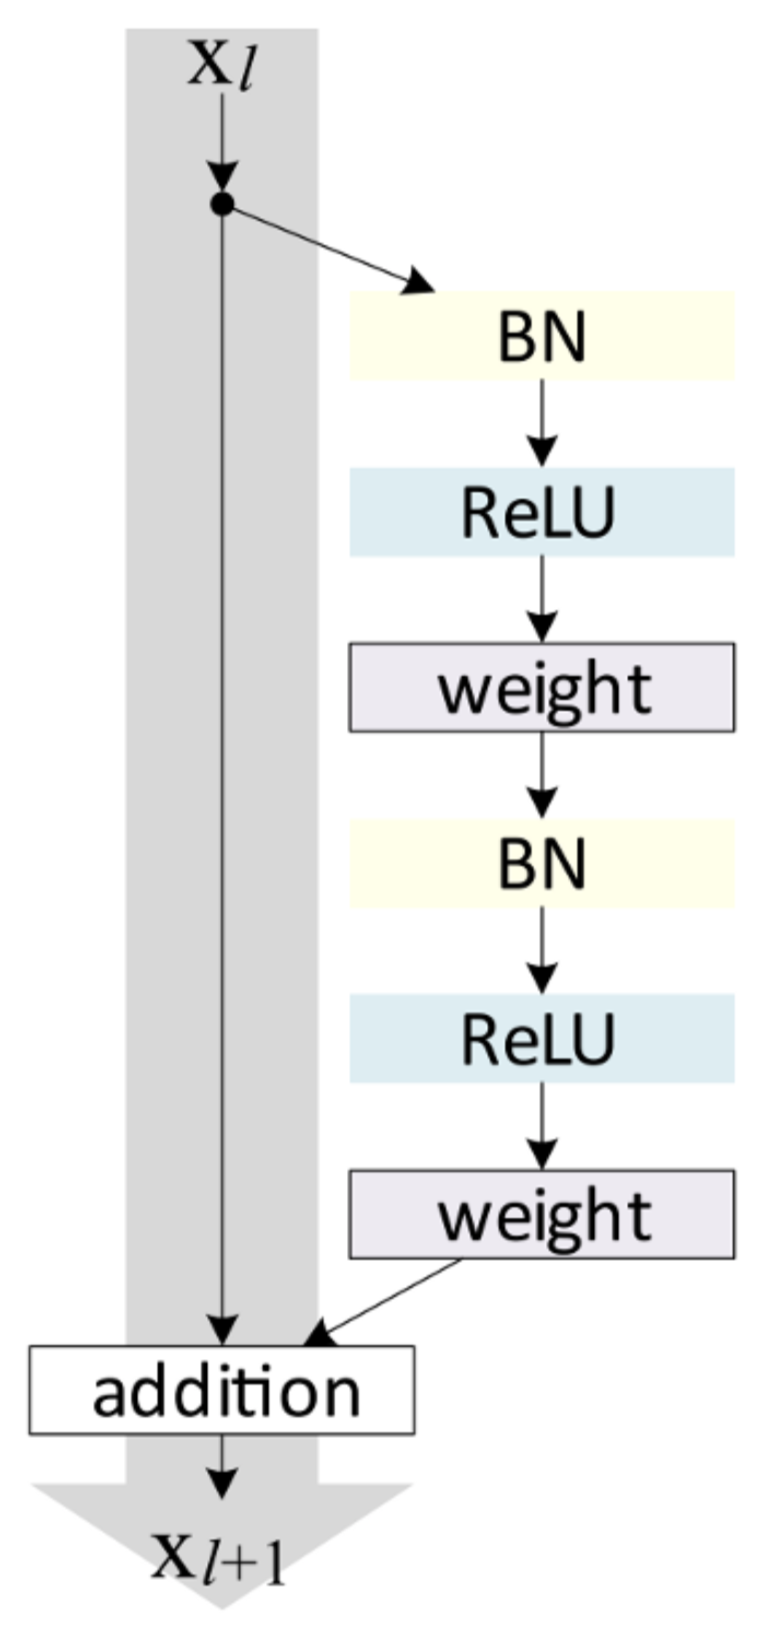
\includegraphics[width = 3.5cm] {resnet.png} \text{\ } 
		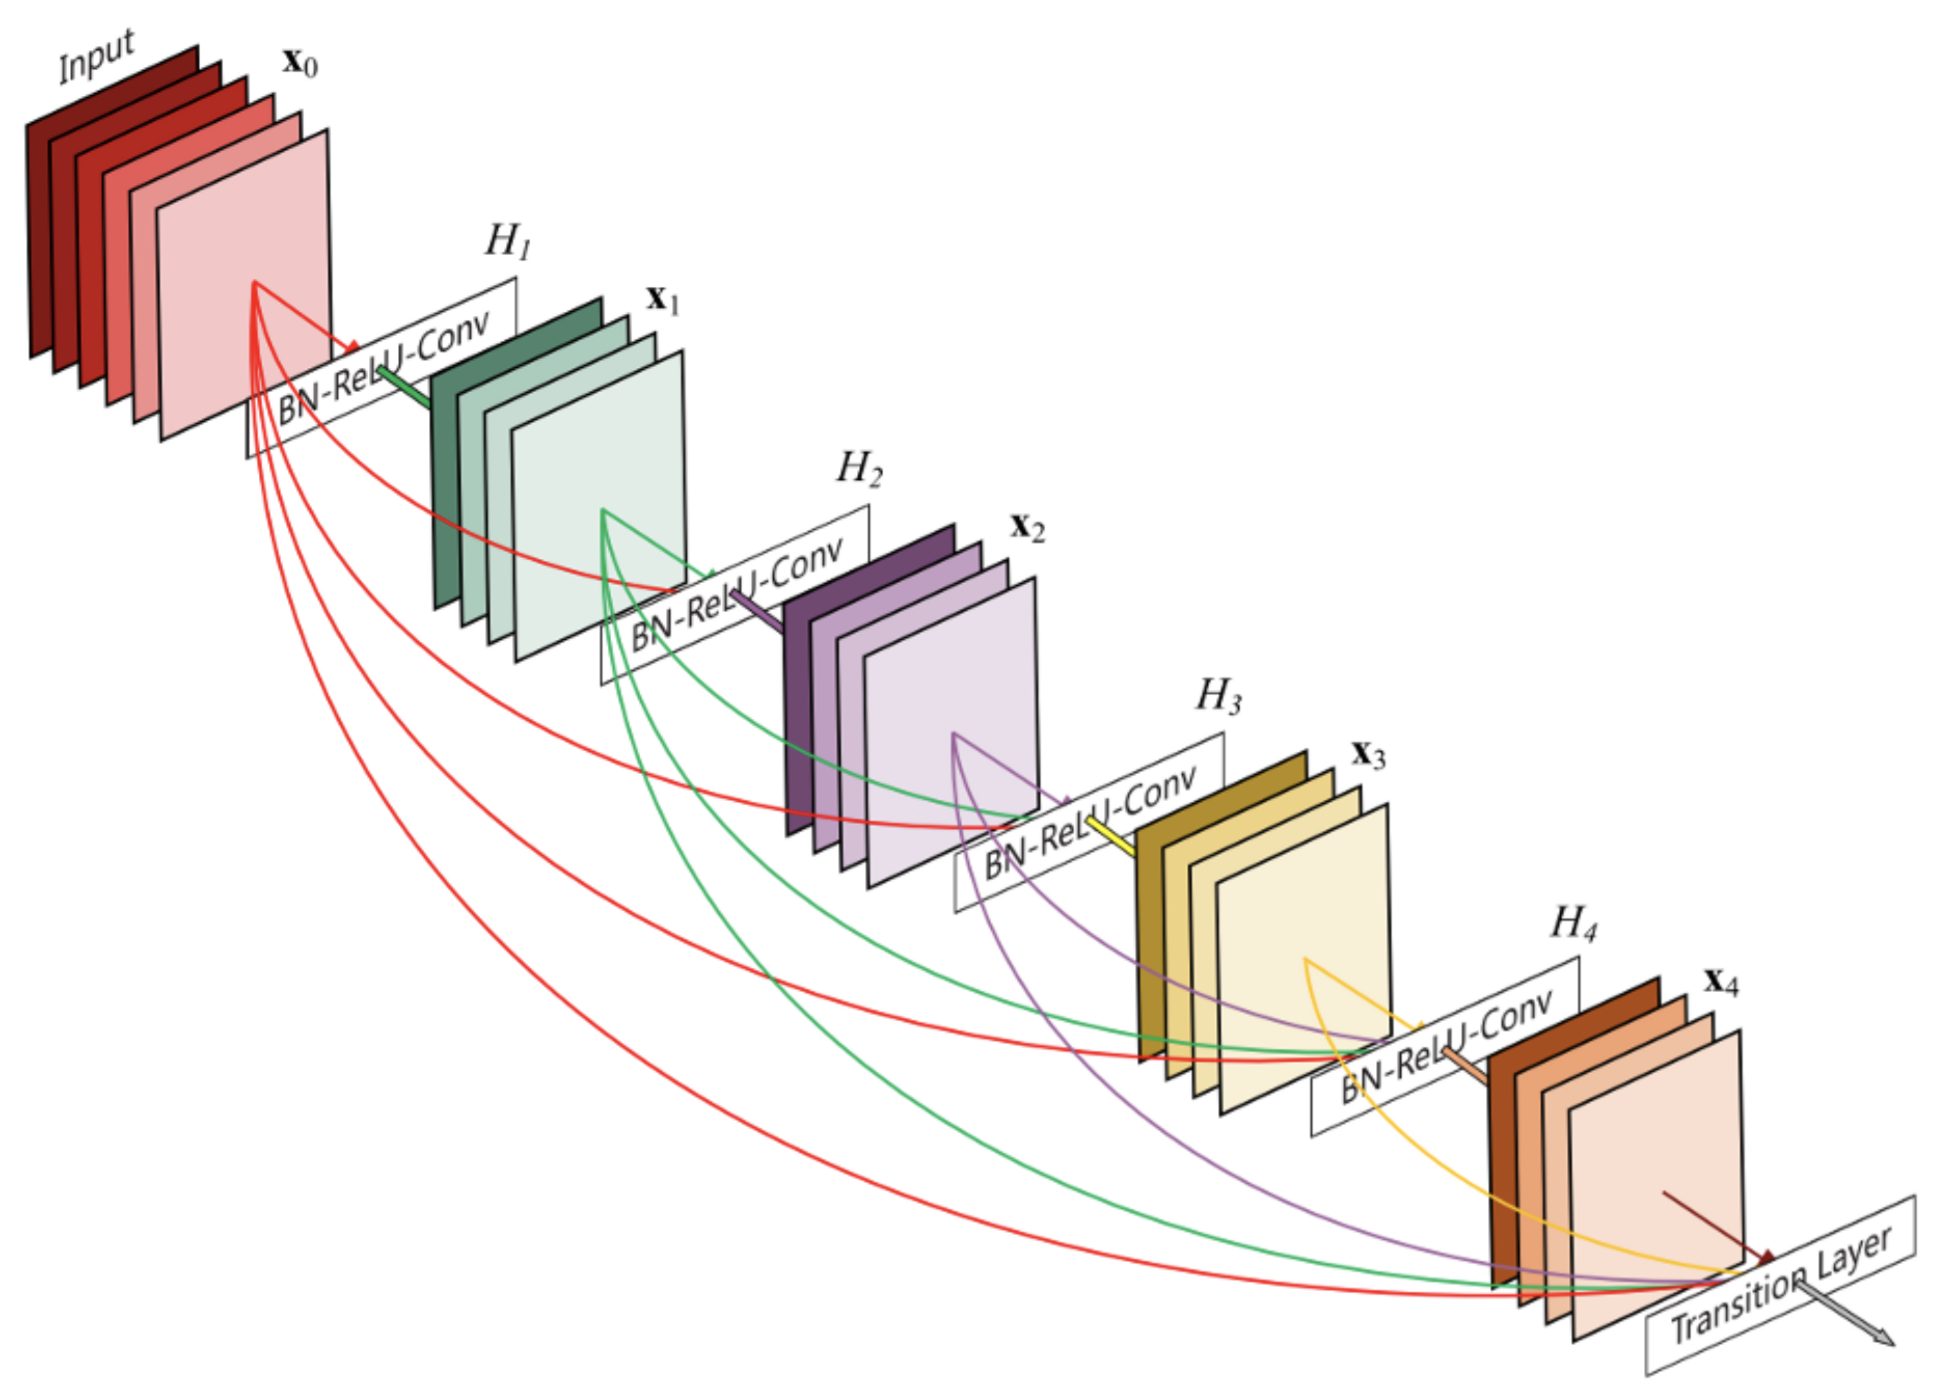
\includegraphics[width = 7cm] {densenet.png} 
		\end{figure} 
	\end{block}
\end{frame}

\begin{frame}
	\begin{block}{Our Experiment}
		\begin{figure}[htbp]
		\centering
		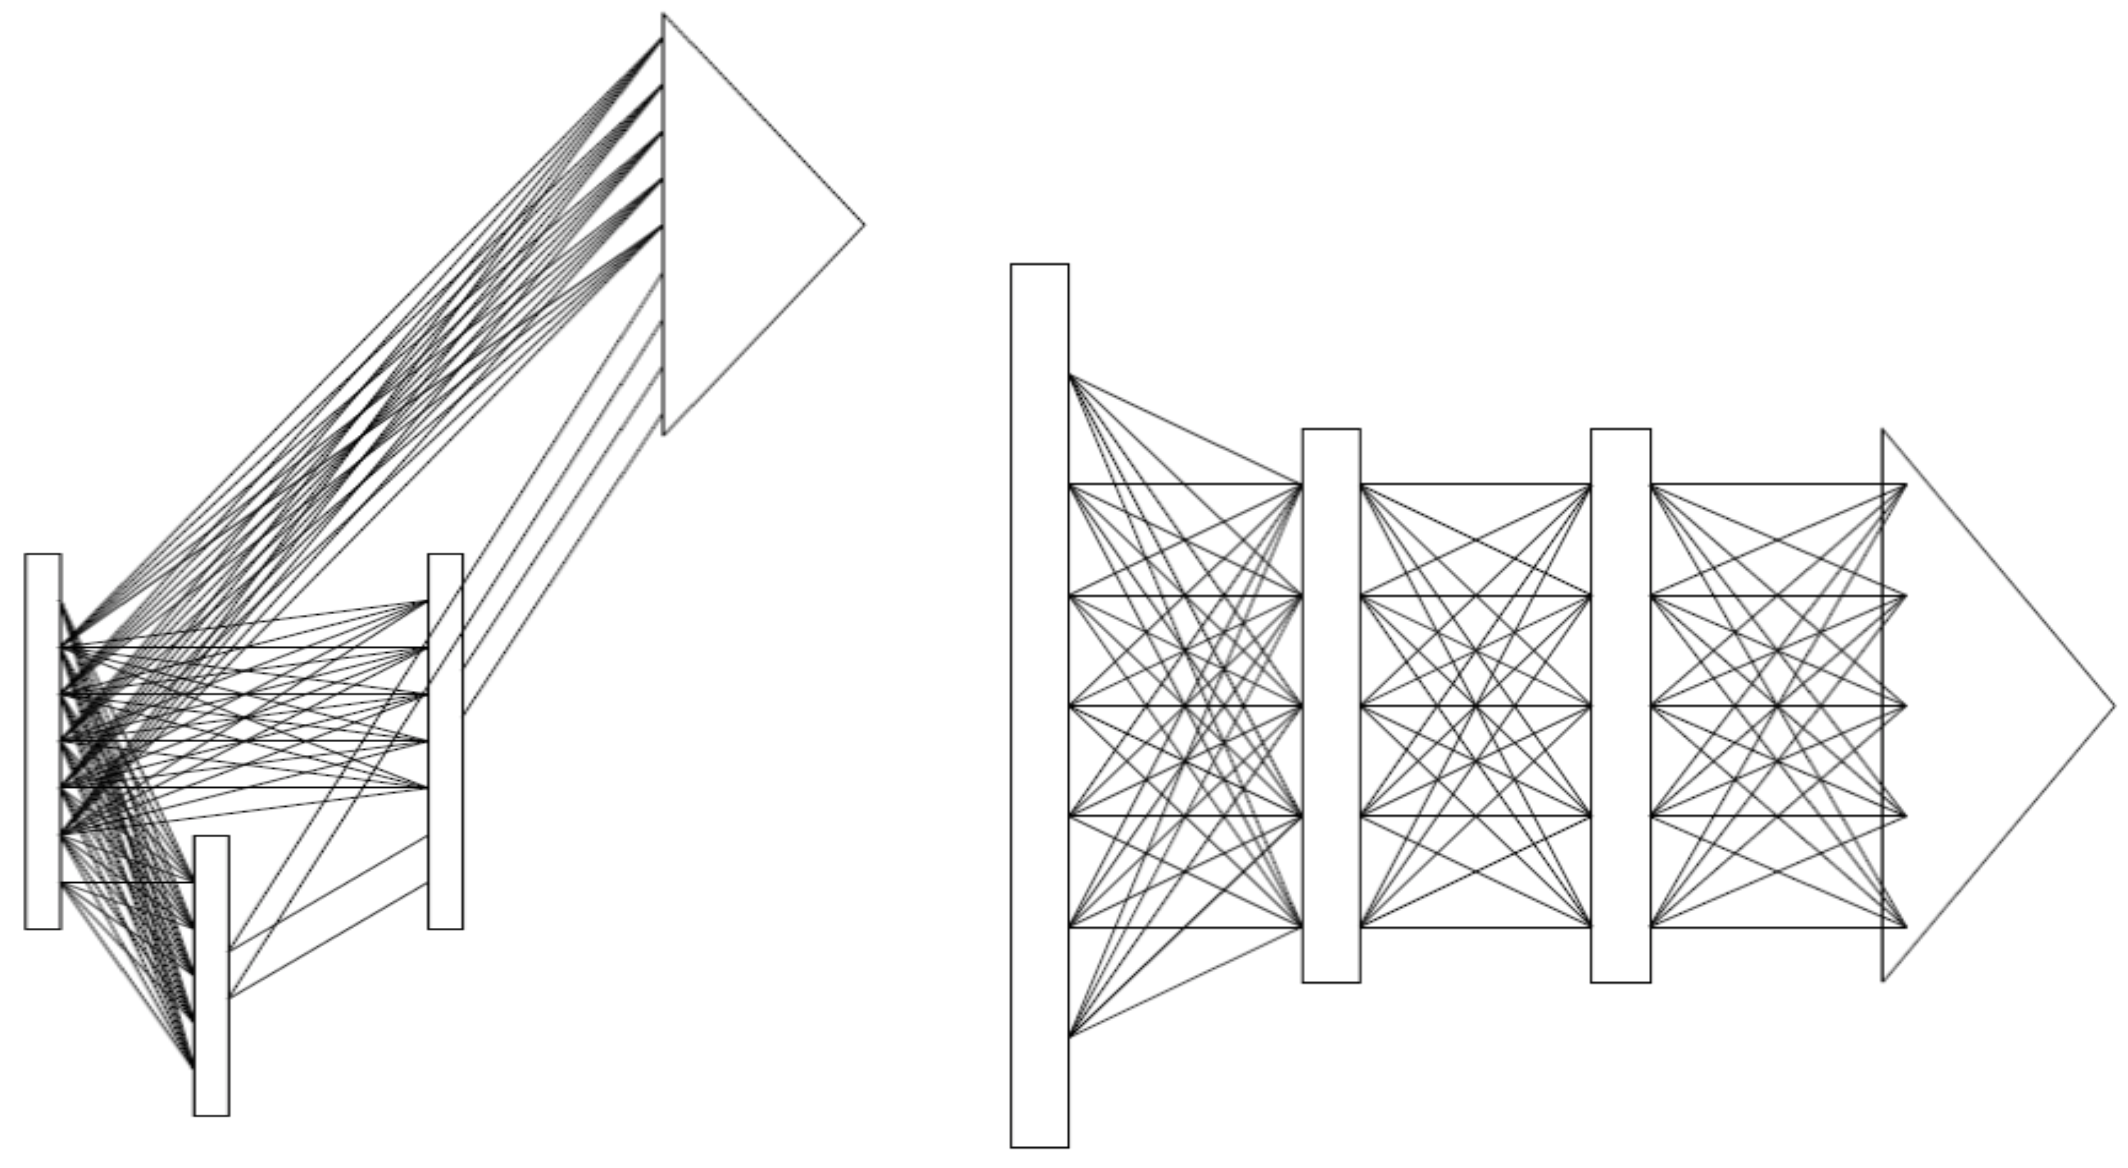
\includegraphics[width = 8cm] {p1.png}
		\end{figure} 
		\begin{itemize}
			\item Compare the performance of two networks.
				\begin{itemize}
				\item better: examine what's in skip connections.
				\item worse: examine why it falls into local minimum.
				\end{itemize}
		\end{itemize}
	\end{block}
\end{frame}

\begin{frame}
	\begin{block}{}
		\centering
		Thanks!
	\end{block}
\end{frame}

\end{document}